%%%%%%%%%%%%%%%%%%%%%%%%%%%%%%%%%%%%%%%%%%%%%%%%%%%%%%%%%%%%%%%%%%%%%%%%%%%%%%%%%%%%%%%%%%
\section{Evaluation}
%%%%%%%%%%%%%%%%%%%%%%%%%%%%%%%%%%%%%%%%%%%%%%%%%%%%%%%%%%%%%%%%%%%%%%%%%%%%%%%%%%%%%%%%%%i
\subsection{Security: do we meet our meet security goals}
   - attack scenarios

\subsection{Performance}

We measure two aspects of \sys's performance: (1) the latency and storage cost of using \sys's
low-level API to apply a disguise, reveal a disguise, or temporarily recorrelate disguised data; and
(2) the impact of these disguising operations on the performance of concurrently executing
application users.

We evaluate performance using three applications: WebSubmit-rs, HotCRP, and Lobsters.

WebSubmit is an answers-submission application for course lectures (similar to \lyt{TODO other
course submission apps}). Its simple schema consists of lectures, questions, answers, and user
accounts; each user owns their account and a set of answers. We integrated \sys into WebSubmit to
support a disguise for admin-anonymization of all answers; a disguise for per-user GDPR-compliant
account deletion; account restoration after deletion; and answer editing after anonymization.
\sys-WebSubmit is a fully-E2E application that supports additional endpoints to perform these
disguise actions, and emails users their capabilities and locators (as these endpoints) when
disguise actions are performed.

\lyt{TODO describe HotCRP and Lobsters.}

\head{Latency Costs of Disguise-Related Actions.}
\begin{table}[t!]
\begin{center}
\begin{tabular}{ c c }
    \textbf{Client Op (20 Lec, 4 Ans/Lec)} & \textbf{Time (ms)}\\
\hline
    Create User Account & 1\\
    Anonymize User Account & 19\\
    Edit Normal Lecture Answer & 2 \\
    Edit Anonymized Lecture Answer & 62 \\
    Delete User Account (Pre-Anon) & 25 \\
    Delete User Account (Post-Anon) & 105 \\
    Restore User Account & 366 \\
\hline
    \textbf{DB Op} & \textbf{Time (ms)}\\
\hline
Update DB Row & 0.1\\ 
Select DB Row (User) & 0.1\\
Remove DB Row (User) & 0.1\\
Select DB Rows (Answers) & 0.2\\
Remove DB Rows (Answers) & 0.2\\
Reveal Deleted Row (DB Select + Insert) & 0.2 \\
Create + Register Principal & 0.1\\
\hline
    \textbf{Crypto Op} & \textbf{Time (ms)}\\
\hline
Generate Keypair & 301\\
Encrypt Ownership Token & 0.4\\
Decrypt Ownership Token & 0.3\\
Encrypt Diff Token & 0.3\\
Decrypt Diff Token & 3.0\\
\end{tabular}
\end{center}
\caption{Amount of time required to run different operations for disguises in WebSubmit. Client operations run on a prepopulated database with 2000 users, 20 lectures, and 4 answers per
    lecture per user, and currently sends requests to the loopback address.}
    \label{tab:opstats}
\end{table}

Table~\ref{tab:opstats} shows the latency of different WebSubmit disguise-related operations.  The
latency of each client operation shown scales linearly with the amount of data (\ie number of
answers) associated with each user. Each client operation requires some number of DB or crypto
operations.

Creating an account in WebSubmit generates an APIKey and registers a private-public keypair for the
user (emailing the user the public key as the user's decryption capability).

Account anonymization generates one pseudoprincipal per lecture, so that all of a user's answers for
a particular lecture belong to the same pseudoprincipal.  Anonymization selects the relevant answers
to anonymize; generates per-lecture pseudoprincipals and ownership tokens; encrypts and stores these
ownership tokens; and performs DB queries to insert pseudoprincipls and to update answer FKs to
point to these new pseudopricipals.

Editing answers normally simply performs update DB queries. Editing anonymized answers, however,
uses client-provided locator and decryption capabilities to authorize the client to speak for the
pseudoprincipal associated with the answer.  \sys performs this authorization check by decrypting
\emph{all} ownership tokens at the specified locator until it finds a ownership token linking the
client to the currently-owning pseudoprincipal. For example, this benchmark's anonymization of a
user account generates 20 ownership token ciphertexts at the same locator; editing anonymized
answers of a single lecture thus performs up to 20 decryptions to determine which pseudoprincipals
the client can act for. This can be optimized by batching all ownership tokens from one disguise
into a single encrypted ciphertext.

Account deletion pre-anonymization does not perform any composition using accessible ownership; \sys
simply selects answers of the user to remove; removes these answers; and encrypts and inserts one
diff token for each answer.

Account deletion post-anonymization first uses a decryption capability and locator to find and
decrypt ownership tokens of the user. This lets \sys find data of pseudoprincipals that the user is
authorized to remove along with their account, and compose account deletion on top of anonymizaton.
\sys decrypts one ownership token for each lecture; selects answers of both the user and any linked
pseudoprincipals to remove; and like before, removes these answers and encrypts and inserts one diff
token for each answer.

Account restoration decrypts a diff token for each answer for each lecture, and performs DB checks
to ensure the diffs can be restored (\eg that the corresponding lecture of an answer to reinsert
still exists). If the checks pass (which they do in this benchmark), restoration reinserts the
answers stored in the diffs.

\head{Storage Costs of Disguise-Related Actions.} Each generated pseudoprincipal adds an additional
row to the users table in WebSubmit; \sys also stores public-key metadata for each principal (and
pseudoprincipal), and (in-memory) encrypted ciphertexts for tokens.  Clients keep track of
capabilities and locators that are emailed to them in the form of URLs that allow for account
restoration or post-anonymization answer editing.

\head{Impact on Normal Application Execution.} Figure~\ref{fig:concurrent} illustrates the
normal-case and worst-case impacts of disguising when WebSubmit has 100 users continuously editing
their lecture answers (in a database containing 2000 users, 20 lectures, and 4 answers per lecture
per user).

To simulate a realistic normal amount of disguising, we imagine that there is always some user in
addition to the 100 editing users that is deleting or restoring their account, and measure the
change in latency. With one disguiser, we observe no increase in latency over the baseline with 0
disguisers (approximately 600ms/edit). 
\lyt{Note the increase from 2ms (for a normal edit) in
Table~\ref{tab:opstats}: this occurs because 100 users (on concurrently running threads)
simultaneously perform nonstop SQL queriest to edit answers, leading to 100\% processor
utilization.}

To simulate the worst-case scenario in practice, we imagine that anywhere from 10 to 25 additional
active users decide to simultaneously delete their account (\eg in response to some social media
campaign). At some later point in time, these users decide to come back and (in the worst case)
restore their accounts simultaneously. We observe that while 10 users disguising themselves at once
has minimal impact on edit latency for the 100 users, 16 users doing so causes
concurrent edit latency spikes up to 1000ms, and 25 users doing so causes spikes up to 2700ms.  
%
These spikes come in pairs, with the larger second spike in the pair coinciding with concurrent
revealing (and the first of the pair coinciding with disguising); revealing has greater impact due
to its higher latency and compute costs.

We imagine \sys can prevent such spikes by rate-limiting and queuing disguise actions when
necessary, in particular for non-time-sensitive disguises like GDPR-compliant account deletion.

\begin{figure}[t!]
    \centering
        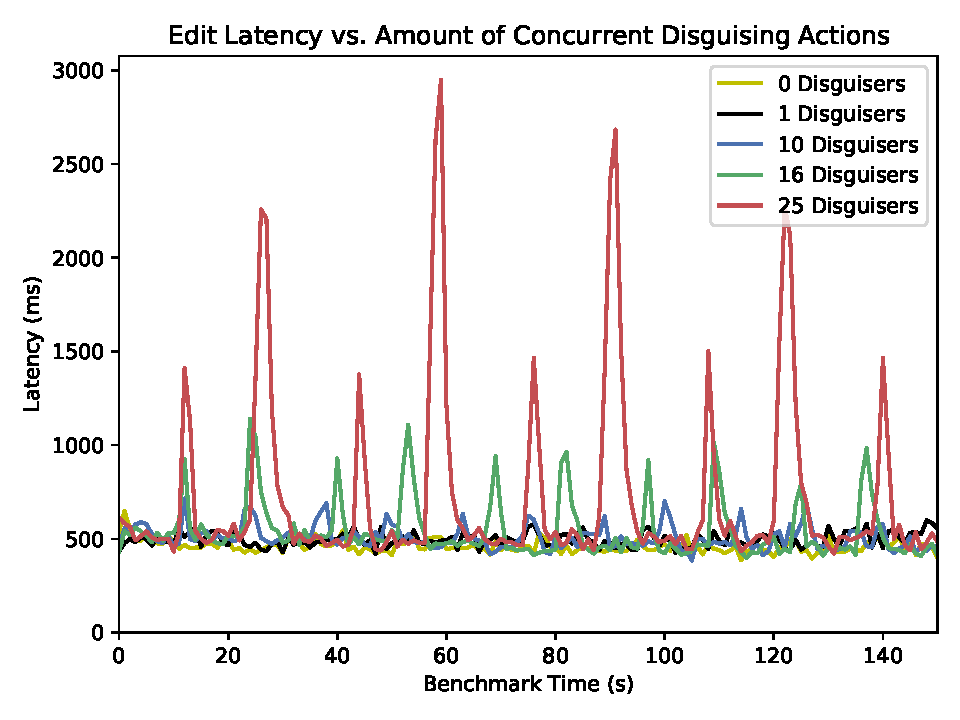
\includegraphics[width=0.5\textwidth]{figs/concurrent_results_20lec_100users}
    \caption{Impact of disguising (account deletion and revealing) on 100 users concurrently running
    normal application answer edits.} 
    \label{fig:concurrent}
\end{figure}

\subsection{Case studies}
   1) websubmit
      - was Edna sufficient for the application's needs?
      - changes to application required (how much work to integrate Edna?)
      - *how* did application use Edna?
        - what disguises?
        - how caps integrated with application?
   2) HotCRP
   3) Lobsters?
   4) Some ecommerce app that requires different types of disguises?
